\documentclass[11pt, a4paper]{article}
\usepackage{pdfpages}
\usepackage{parallel}
\usepackage[T2A]{fontenc}
\usepackage{ucs}
\usepackage[utf8x]{inputenc}
\usepackage[polish,english,russian]{babel}
\usepackage{hyperref}
\usepackage{rotating}
\usepackage[inner=2cm,top=1.8cm,outer=2cm,bottom=2.3cm,nohead]{geometry}
\usepackage{listings}
\usepackage{graphicx}
\usepackage{wrapfig}
\usepackage{longtable}
\usepackage{indentfirst}
\usepackage{array}
\usepackage{tikzsymbols}
\usepackage{soul}
\usepackage[ruled,vlined]{algorithm2e}
%\counterwithout{figure}{section} 

\usepackage{url}
\makeatletter
\g@addto@macro{\UrlBreaks}{\UrlOrds}
\makeatother

\newcolumntype{P}[1]{>{\raggedright\arraybackslash}p{#1}}
\frenchspacing
\usepackage{fixltx2e} %text sub- and superscripts
\usepackage{icomma} % коскі ў матэматычным рэжыме
\PreloadUnicodePage{4}

\newcommand{\longpage}{\enlargethispage{\baselineskip}}
\newcommand{\shortpage}{\enlargethispage{-\baselineskip}}

\def\switchlang#1{\expandafter\csname switchlang#1\endcsname}
\def\switchlangbe{
\let\saverefname=\refname%
\def\refname{Літаратура}%
\def\figurename{Іл.}%
}
\def\switchlangen{
\let\saverefname=\refname%
\def\refname{References}%
\def\figurename{Fig.}%
}
\def\switchlangru{
\let\saverefname=\refname%
\let\savefigurename=\figurename%
\def\refname{Литература}%
\def\figurename{Рис.}%
}

\hyphenation{admi-ni-stra-tive}
\hyphenation{ex-pe-ri-ence}
\hyphenation{fle-xi-bi-li-ty}
\hyphenation{Py-thon}
\hyphenation{ma-the-ma-ti-cal}
\hyphenation{re-ported}
\hyphenation{imp-le-menta-tions}
\hyphenation{pro-vides}
\hyphenation{en-gi-neering}
\hyphenation{com-pa-ti-bi-li-ty}
\hyphenation{im-pos-sible}
\hyphenation{desk-top}
\hyphenation{elec-tro-nic}
\hyphenation{com-pa-ny}
\hyphenation{de-ve-lop-ment}
\hyphenation{de-ve-loping}
\hyphenation{de-ve-lop}
\hyphenation{da-ta-ba-se}
\hyphenation{plat-forms}
\hyphenation{or-ga-ni-za-tion}
\hyphenation{pro-gramming}
\hyphenation{in-stru-ments}
\hyphenation{Li-nux}
\hyphenation{sour-ce}
\hyphenation{en-vi-ron-ment}
\hyphenation{Te-le-pathy}
\hyphenation{Li-nux-ov-ka}
\hyphenation{Open-BSD}
\hyphenation{Free-BSD}
\hyphenation{men-ti-on-ed}
\hyphenation{app-li-ca-tion}

\def\progref!#1!{\texttt{#1}}
\renewcommand{\arraystretch}{2} %Іначай формулы ў матрыцы зліпаюцца з лініямі
\usepackage{array}

\def\interview #1 (#2), #3, #4, #5\par{

\section[#1, #3, #4]{#1 -- #3, #4}
\def\qname{LVEE}
\def\aname{#1}
\def\q ##1\par{{\noindent \bf \qname: ##1 }\par}
\def\a{{\noindent \bf \aname: } \def\qname{L}\def\aname{#2}}
}

\def\interview* #1 (#2), #3, #4, #5\par{

\section*{#1\\{\small\rm #3, #4. #5}}
\ifx\ParallelWhichBox\undefined%
    \addcontentsline{toc}{section}{#1, #3, #4}%
\else%
\ifnum\ParallelWhichBox=0%
    \addcontentsline{toc}{section}{#1, #3, #4}%
\fi\fi%

\def\qname{LVEE}
\def\aname{#1}
\def\q ##1\par{{\noindent \bf \qname: ##1 }\par}
\def\a{{\noindent \bf \aname: } \def\qname{L}\def\aname{#2}}
}

\newcommand{\interviewfooter}[1]{
\vskip 1em
\noindent \textit{#1}
}


\begin{document}

\title{1995 "--- Mouse Systems ProAgio / Genius EasyScroll Mouse}
\date{}
\maketitle

Мышь Genius EasyScroll, известная также как Mouse Systems ProAgio Scroll Mouse "--- первая серийно выпускавшаяся мышь с колесом прокрутки. Мышь была выпущена в 1995 году, через пять лет после приобретения Mouse Systems компанией KYE, владельцем торговой марки Genius.

\begin{figure}[h]
    \centering
    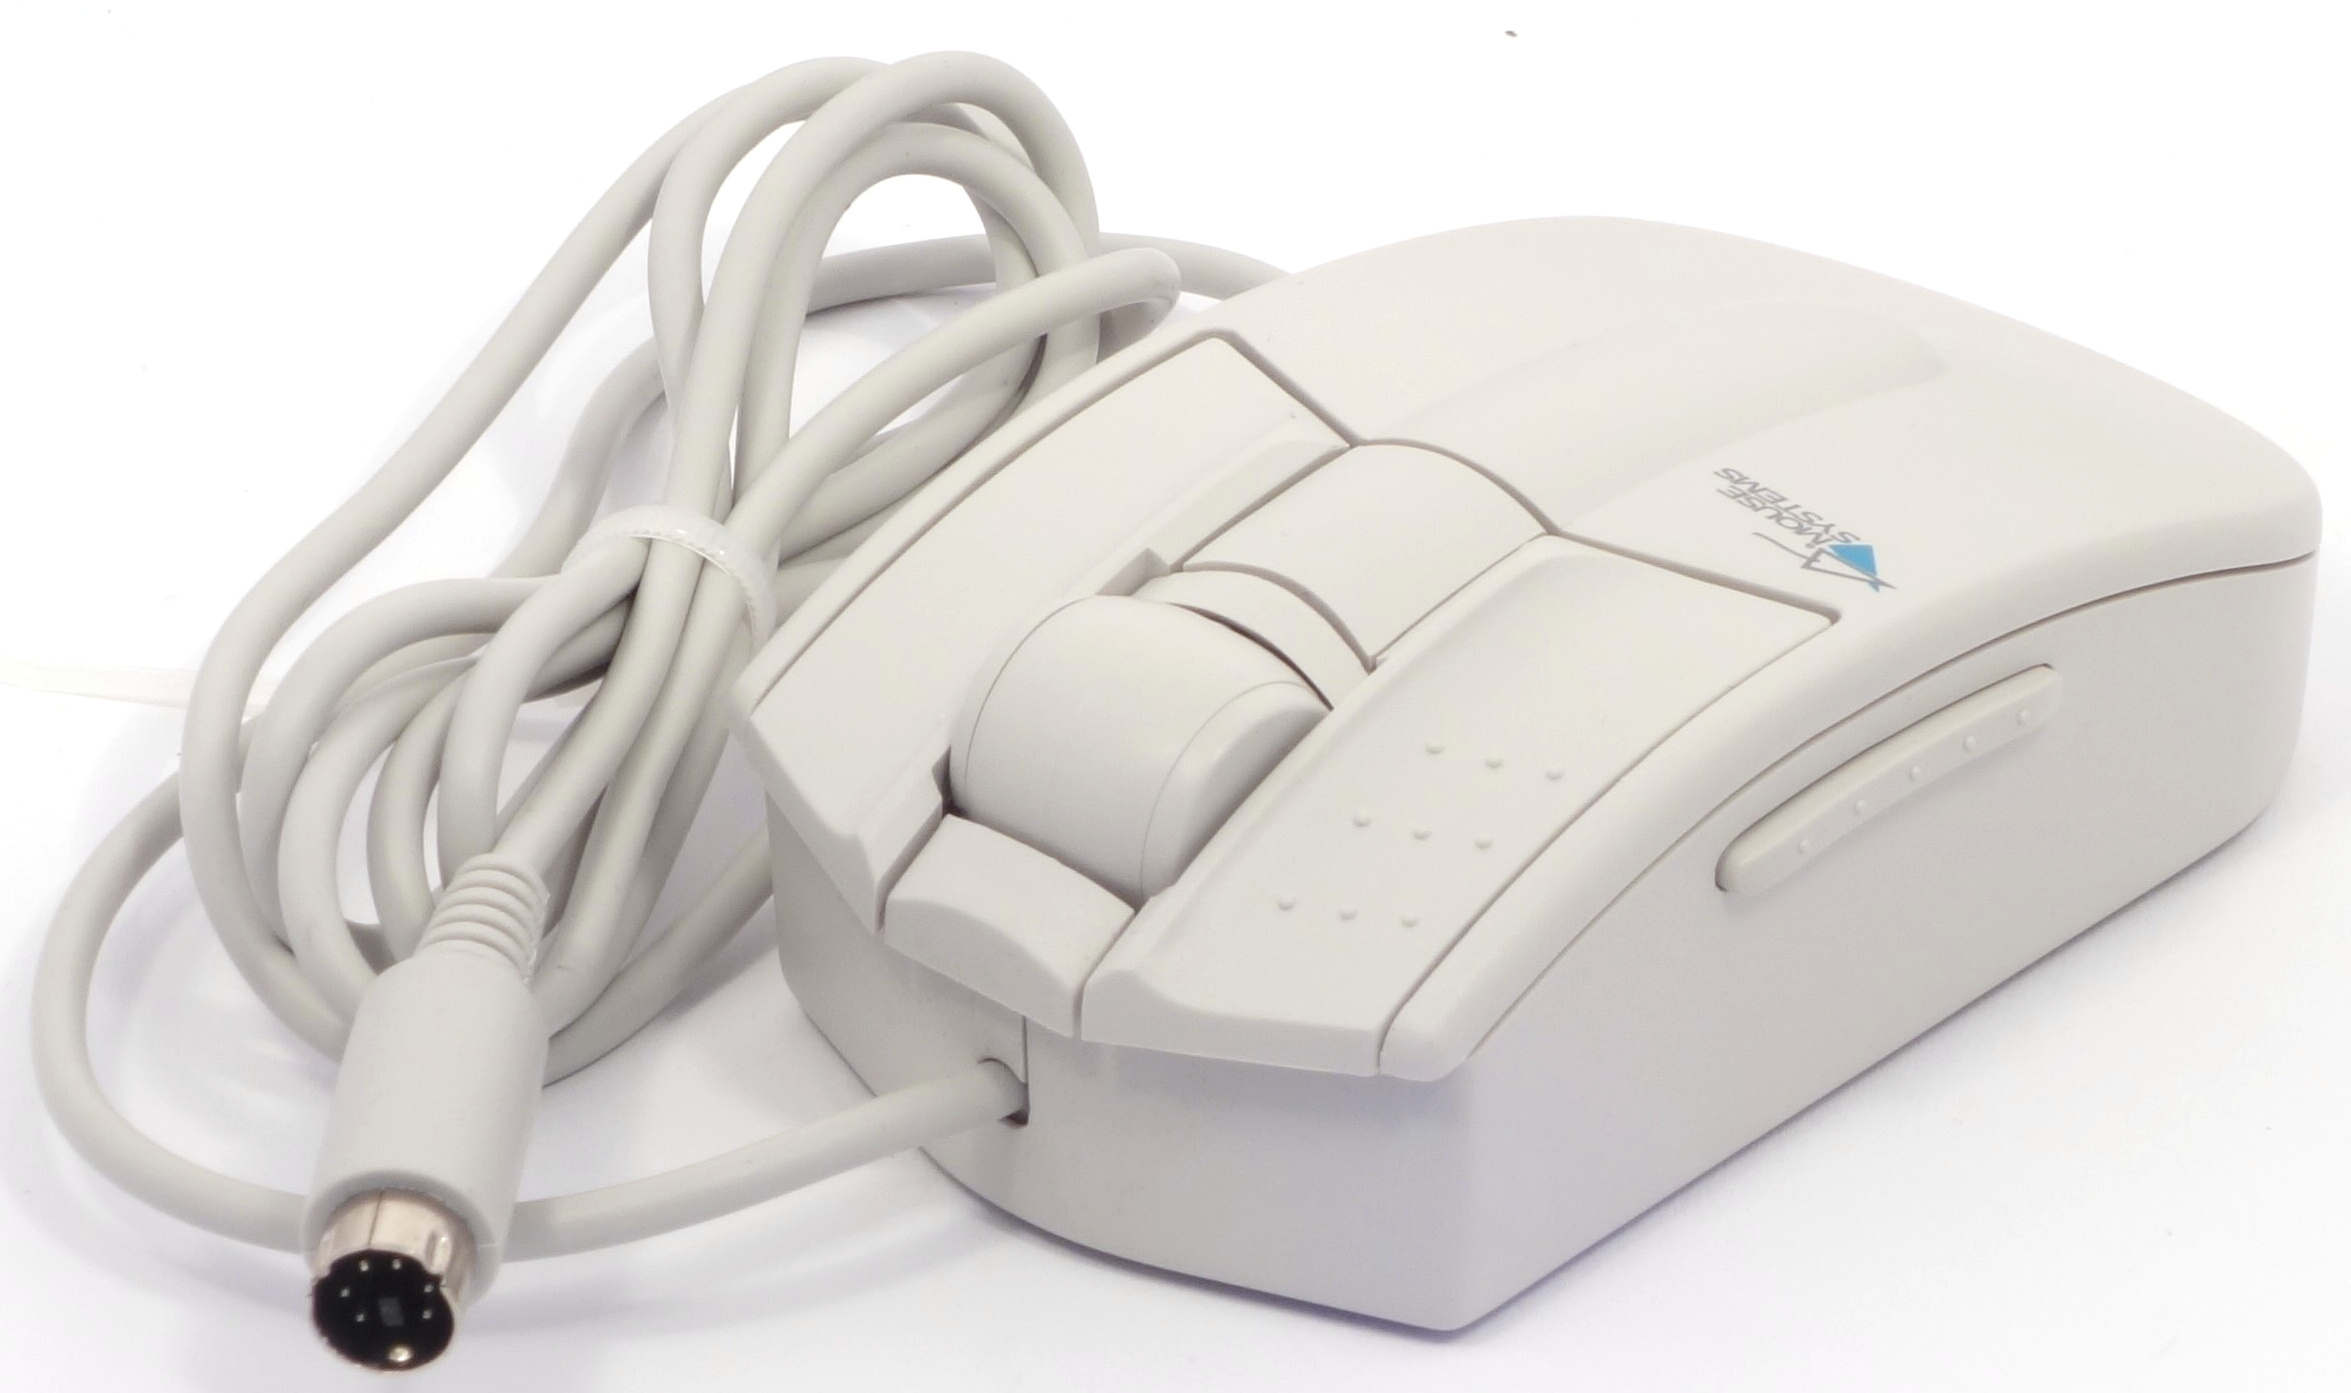
\includegraphics[scale=0.5]{1995_pro_agio_scroll_mouse/pic_30.jpg}
    \caption{ProAgio Scroll Mouse}
    \label{fig:ScrollPic}
\end{figure}


Мышь имеет эргономичную форму (рис. \ref{fig:ScrollPic}). Устройство оснащено пятью кнопками, которые имеют достаточно большую площадь и ребристые края, а левая кнопка снабжена рельефной поверхностью для более легкой тактильной идентификации. Колесо прокрутки расположено посередине корпуса в его дальней от пользователя части, и оно намного шире, чем в более поздних версиях (фактически, это можно было бы назвать не колесом, а роликом или барабаном). Помимо функции прокрутки, оно реагирует на нажатие как на кнопку, как у большинства более поздних мышей. Также пользователю доступна для нажатия большим пальцем вытянутая узкая кнопка на боковой стороне корпуса \ref{fig:ScrollHand}. Предположительно, функции кнопок можно переназначать с помощью программного обеспечения \cite{yt}.

\begin{figure}[h]
    \centering
    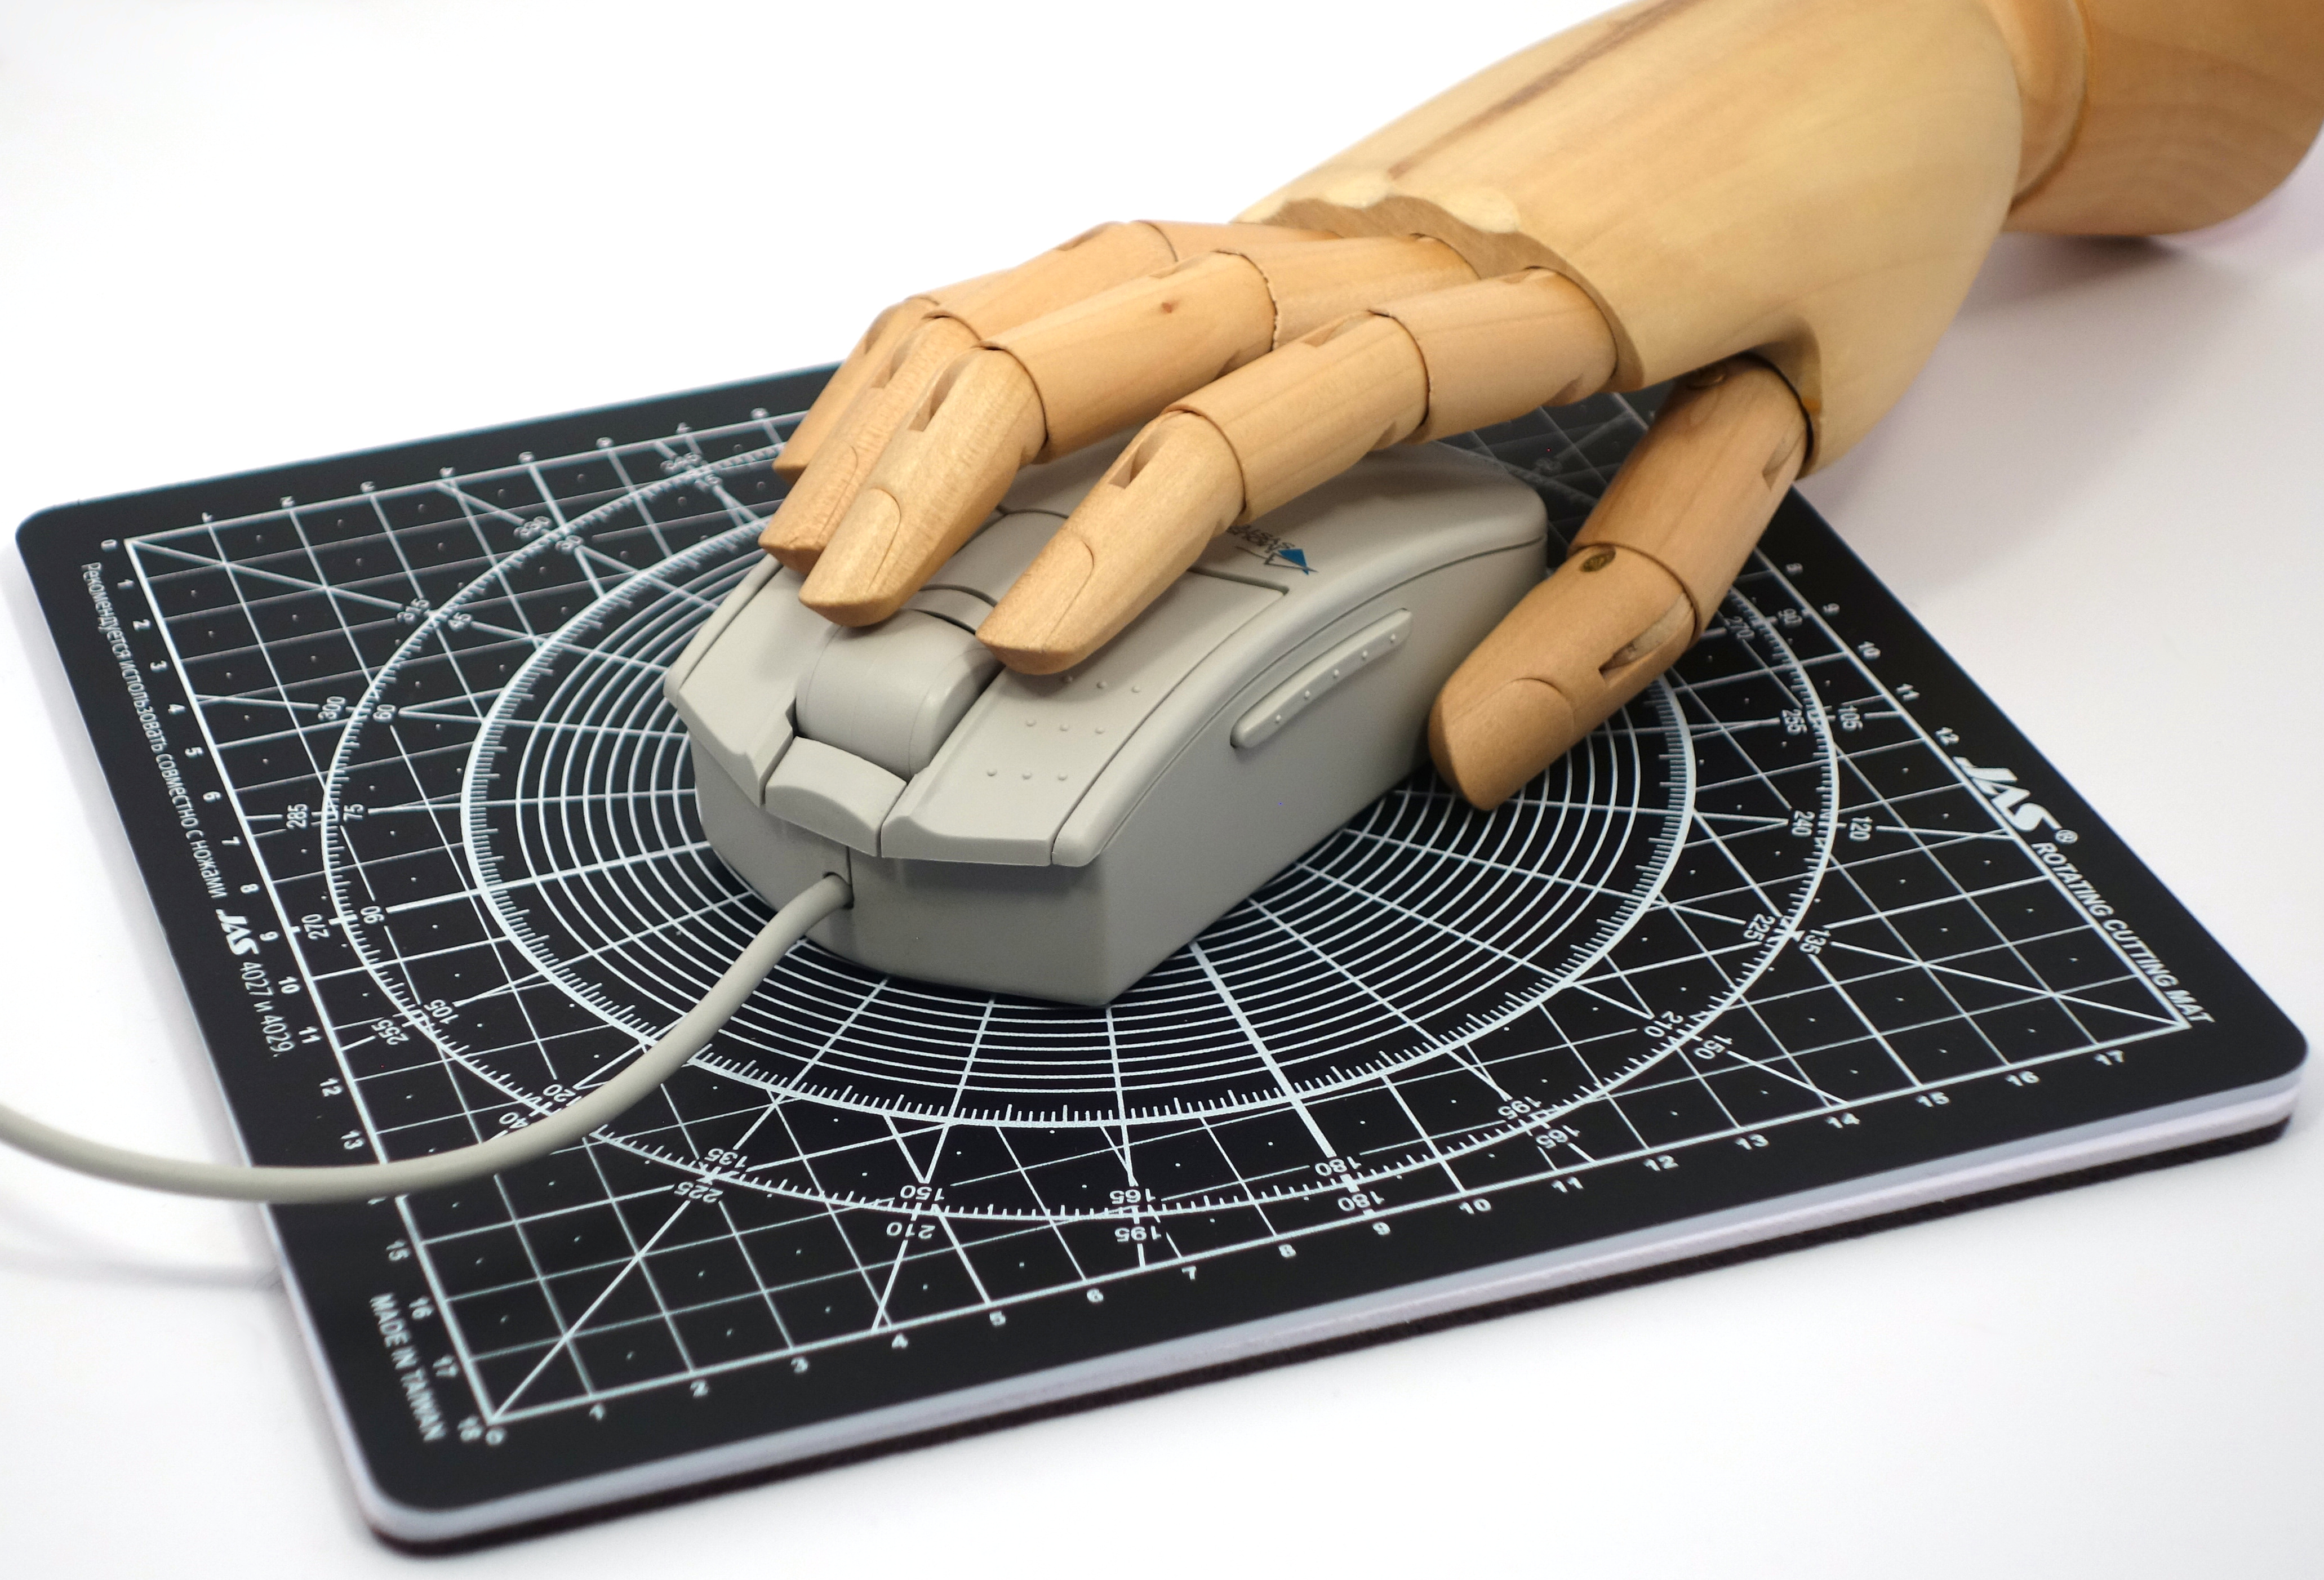
\includegraphics[scale=0.3]{1995_pro_agio_scroll_mouse/hand_30.jpg}
    \caption{Изображение ProAgio Scroll Mouse с моделью руки человека}
    \label{fig:ScrollHand}
    \end{figure}

Стоит отметить, что идея вращаемого пальцем ролика на указательном устройстве появилась раньше, чем ProAgio Scroll Mouse, но оно никогда прежде не использовалось для прокрутки текста. Например, разработчики трекбола MicroSpeed FastTRAP в 1987 году использовали колесо в качестве средства перемещения по координатной оси \textit{z} в программах, связанных с трехмерной графикой (в то время, как шар трекбола традиционно обеспечивал перемещение по осям \textit{x} и \textit{y}). В информационных материалах по FastTRAP, выпущенных MicroSpeed, колесо описывалось как «Trackwheel для указания третьей оси».

\begin{figure}[h]
    \centering
    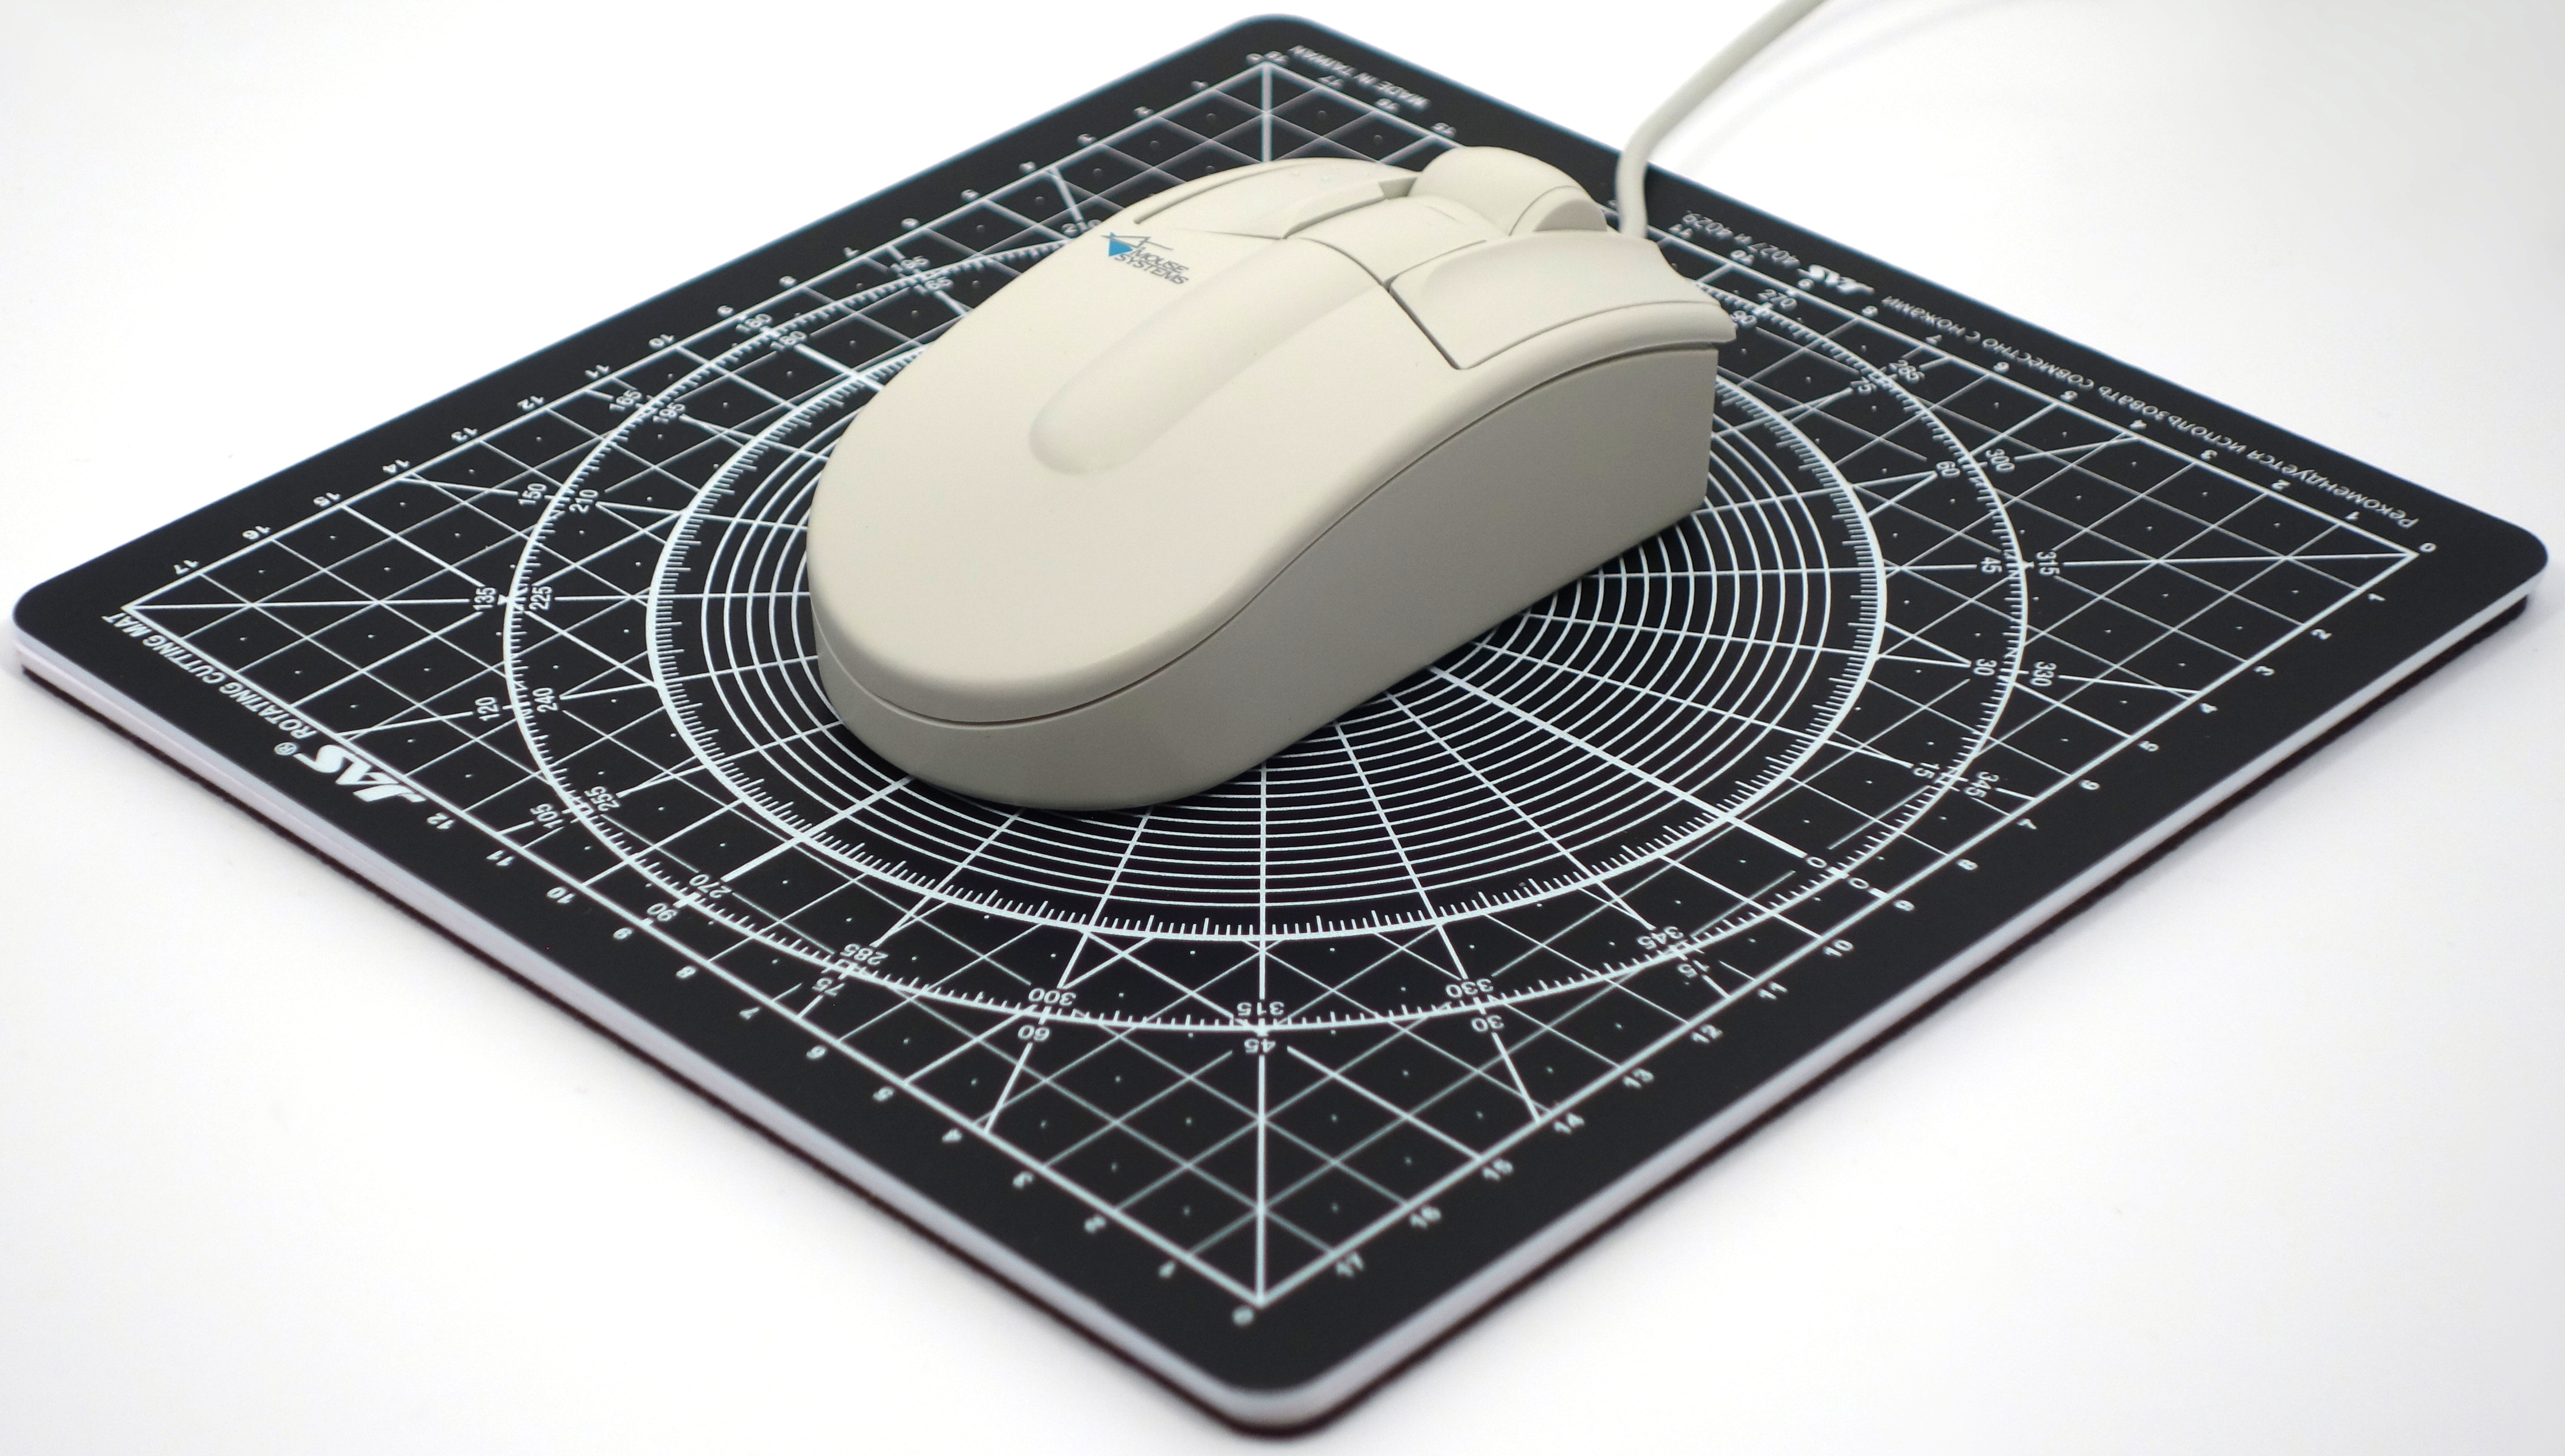
\includegraphics[scale=0.37]{1995_pro_agio_scroll_mouse/size_30.jpg}
    \caption{Изображение ProAgio Scroll Mouse на размерном коврике с шагом сетки 1~см}
    \label{fig:ScrollSize}
\end{figure}

Процитируем Эрика Мишельмана из компании Microsoft, расскрывающего особенности его появления в статье История колеса прокрутки \cite{ink}:

\textit{<<Еще в 1993 году, когда я наблюдал, как многие пользователи Excel выполняют свою работу, я заметил, что им сложно перемещаться в больших электронных таблицах. Поиск и переход в разные разделы часто доставлял трудности. У меня была мысль, что здесь может помочь более продвинутое устройство ввода.
Моей первоначальной идеей был рычаг зума. Это был просто рычаг, предположительно для вашей руки, не связанной с мышью (то есть слева от клавиатуры, если вы правша). Когда вы отталкиваете рычаг от себя, размер таблицы уменьшается, а когда вы тянете его к себе, выполняется приближение.}

\textit{Я прототипировал эту идею, подключив джойстик к моему компьютеру и используя DDE, чтобы подключить его к Excel для масштабирования. Используя кнопку джойстика вместе со стиком, я также заставил его выполнять <<масштабирование данных>>, углубляясь и выходя из контуров Excel.}

\textit{Все это показалось мне полезным, поэтому я показал это подразделению аппаратного обеспечения Microsoft. Первоначально они относились к идее, которую я представил как рычаг зума, как к никуда не годной.}

\textit{В тот момент большинство людей сочло это странным. Но сосредоточение внимания на масштабировании было подходом, очень ориентированным на Excel. В частности, это был <<очень двумерный>> подход. То есть, используя приложение, которое представляет двумерные данные, такие как электронная таблица или графика, очень полезно увеличивать и уменьшать масштаб. Но основной стиль многих других приложений "--- это линейный поток данных, как в Word, и в таких приложениях эта функция не настолько полезна. Вы можете выполнять масштабирование в Word, где уменьшение масштаба показывает вам многостраничный вид, а затем вы щелкаете нужную страницу и увеличиваете ее, но это не так естественно, как с электронной таблицей или графическими изображениями.}

\textit{Некоторые люди предложили добавить функции панорамирования и прокрутки. В частности, я помню, как Крис Грэм сказал, что масштабирование слишком ограничивает, и нужно также использовать панорамирование. В ответ на эти отзывы я добавил панорамирование к прототипу, поэтому, перемещая джойстик из стороны в сторону и вперед-назад, Excel мог прокручивать таблицу в соответствующем направлении.}

\textit{Примерно в это время специалисты по аппаратному обеспечению включились в обсуждение и сообщили, что они рассматривали возможность добавления колесика к мыши, но не знали, для чего оно могло бы использоваться. Навигация по документам как раз была ответом на этот вопрос, поэтому они сказали, что если бы я мог заставить Office поддерживать эту функцию, они бы ее реализовали. На самом деле речь шла о поддержке в приложениях Excel и Word, поскольку они были <<гориллами весом 800 фунтов>> "--- если Excel и Word что-то поддерживали, то другие приложения Office следовали за ними, а если Office в целом что-то поддерживает, то все остальные тоже идут следом (это было начало 1993 года, когда Office был основной причиной использования компьютеров большинством людей)>>.}

\begin{figure}[h]
    \centering
    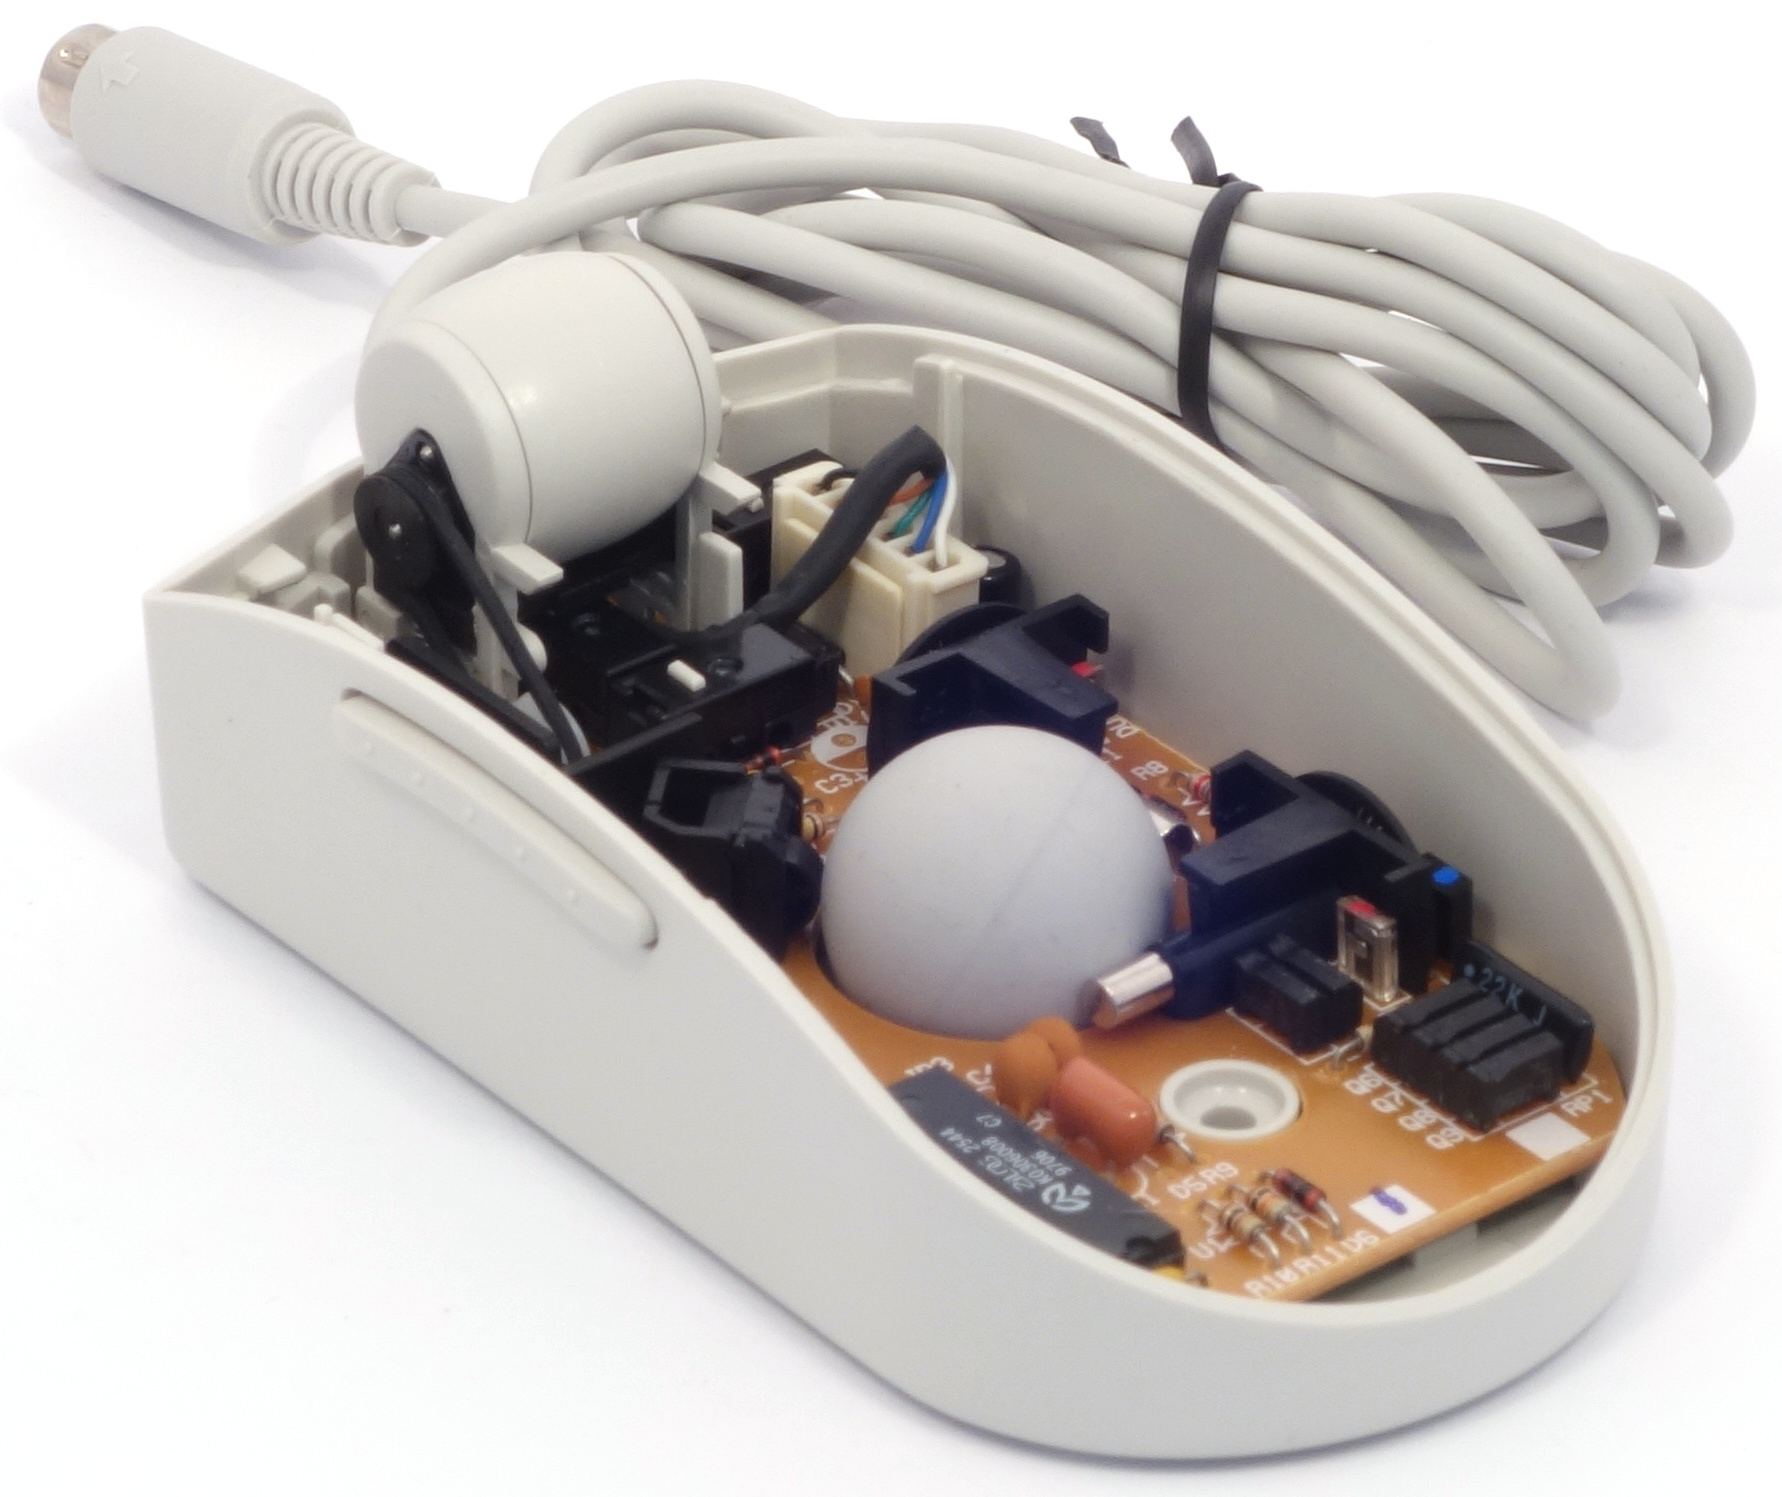
\includegraphics[scale=0.8]{1995_pro_agio_scroll_mouse/inside_30.jpg}
    \caption{Изображение ProAgio Scroll Mouse в разобранном виде}
    \label{fig:ScrollInside}
\end{figure}

Изображение ProAgio Scroll Mouse в разобранном виде показано на рисунке \ref{fig:ScrollInside}. Как можно видеть, мышь использует оптико-механическую технологию (разрешение составляет 400 точек на дюйм). Также среди особенностей следует отметить, что для передачи вращения колеса разработчики использовали ременную передачу на основе резинового пасика, что никогда не встречается в более современных устройствах.

\begin{thebibliography}{9}
\bibitem {ink} CODING HORROR \url{https://blog.codinghorror.com/meet-the-inventor-of-the-mouse-wheel/}
\bibitem {yt} Mouse Systems ProAgio Scroll Mouse \url{https://www.oldmouse.com/mouse/mousesystems/scroll.shtml}
\end{thebibliography}
\end{document}
